\documentclass[
  11pt,
  letterpaper,
   addpoints,
   answers
  ]{exam}

\usepackage{../exercise-preamble}

\begin{document}

\noindent
\begin{minipage}{0.47\textwidth}

\includegraphics[width=\textwidth]{../fcfm_die}
\end{minipage}
\begin{minipage}{0.53\textwidth}
\begin{center} 
\large\textbf{Fundamentos de control de sistemas} (EL4111-1) \\
\large\textbf{Clase auxiliar 3} \\
\small Prof.~Roberto Cardenas Dobson\\
\small Prof.~Aux.~Osvaldo Jimenez - Erik Sáez\\
\small Ayudantes.~Simon Arenas- Juan Pablo Baez - Francisco Garces - Sofia Ibarra\\
\end{center}
\end{minipage}

\vspace{0.5cm}
\noindent
\vspace{.85cm}

\begin{questions}
    %%%%%%%%%%%%%%%%%%%%%%%%%%%
    \question Considere el siguiente sistema de control:
    \begin{figure}[h]
        \centering
        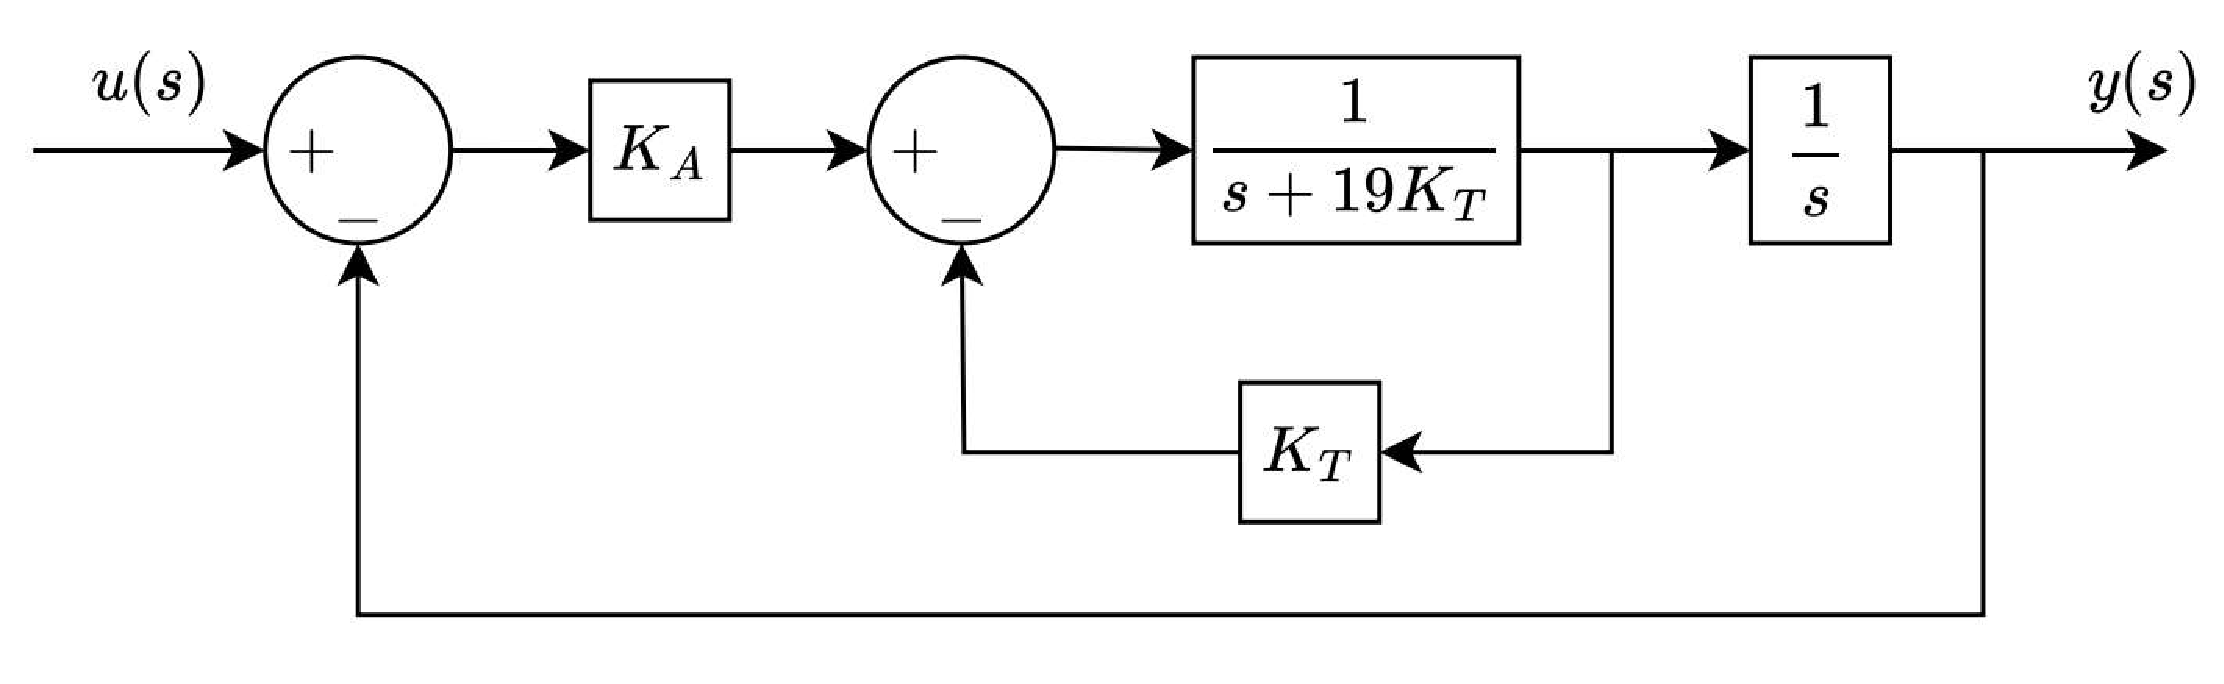
\includegraphics[width=0.7\textwidth]{Auxiliar_3_1}
        \caption{Diagrama de bloques}
    \end{figure}
    \begin{enumerate}
        \item Encuentre los valores de $K_T$ y $K_A$ requeridos para lograr cero error en estado estacionario a entrada escalón. Dichos valores deben permitir alcanzar una respuesta con un $\xi = 0.707$ y una $\omega_n = 20 \, \text{rad/seg}$. Resuelva el problema de forma gráfica, apoyándose en las condiciones de módulo y de ángulo.
        \item Debido a una deficiente implementación en el microprocesador, el integrador toma la forma de la planta $\frac{s-10K_A}{5sK_A}$. Incluso con este error, ¿Es posible diseñar un sistema de control que sea estable? Si así lo cree, determine las condiciones necesarias sobre $K_A$ para que la respuesta del sistema sea estable. \textbf{HINT:} Analice como varía el LGR para distintos valores de $K_A$.
        \item Suponga que el sistema de control experimenta una entrada del tipo $u(t) = 400 + 60 \cos (\omega_0 t) + 2t$, con $\omega_0$ una frecuencia de resonancia constante ¿Cómo modificaría usted el controlador $K_A$ para alcanzar cero error en estado estacionario para dicha entrada?
    \end{enumerate}
    
%%%%%%%%%%%%%%%%%%%%%%%%%%%
\begin{solution}
\subsection*{Resolucion 1.1}
Encuentre los valores de $K_T$ y $K_A$ requeridos para lograr cero error en estado estacionario a entrada escalón. Dichos valores deben permitir alcanzar una respuesta con un $\xi=0.707$ y una $\omega_n=20 rad/seg$. Resuelva el problema de forma gráfica, apoyándose en las condiciones de módulo y de ángulo.

En primera instancia, resolvemos el lazo interno del sistema de control. Utilizando la función de transferencia de lazo cerrado se obtiene lo siguiente:
\begin{align}
    G_{int}(s)&=\frac{\frac{1}{s+19K_T}}{1+ \frac{K_T}{s+19K_T}} \nonumber \\
    &=\frac{\frac{1}{s+19K_T}}{\frac{s+19K_T+K_T}{s+19K_T}} \nonumber \\
    &=\frac{1}{s+20K_T} \nonumber
\end{align}

De esta forma, la función a lazo abierto del sistema de control queda de la siguiente forma:
\begin{equation}
    G(s)H(s)=\frac{K_A}{s(s+20K_T)} \nonumber
\end{equation}

El punto de diseño, por otra parte, estará dado por:
\begin{align}
    s_{1,2}^* &=-\xi\omega_n \pm j\omega_n\sqrt{1-\xi^2} \nonumber \\
    &=-0.707\cdot20\pm j20\sqrt{1-0.707^2} \nonumber \\
    &=-14.14\pm j 14.14
\end{align}
A partir de lo anterior, podemos construir el LGR del sistema de control. Notar que la función de lazo abierto presenta únicamente 2 polos. Por ende, el lugar de corte de las asíntotas corresponderá al punto medio entre la posición de dichos polos. De esta forma, la posición de las asíntotas será  $\sigma_A=\frac{-20K_T-0}{2}=-10K_T$. Finalmente, el LGR se ve de la siguiente forma:


Dado que existe LGR sobre las asíntotas, el punto de diseño debe ubicarse sobre las mismas, puesto que es el único lugar en donde los polos de lazo cerrado pueden tener una parte imaginario distinta de cero. De esta forma, utilizando el hecho de que el punto de diseño y la posición de las asíntotas tienen la misma ubicación en el eje real:
\begin{align}
    \sigma_A&=-\xi\omega_n \nonumber\\
    -10K_T&=-14.14\\
    K_T&=1.414 
\end{align}

De la anterior ya se tiene el valor de $K_T$. Por otro lado, para encontrar le valor de $K_A$, basta con aplicar la condición de módulo en el LGR. En este sentido, se puede calcular la ganancia de manera geométrica, considerando las distancias desde los polos hasta el punto de diseño. Para calcular esto, se puede hacer de dos formas:
\begin{enumerate}
    \item La distancia que tiene el polo del origen hacia el punto de diseño se puede calcular mediante el teoremas de pitágoras. De esta forma, $d_1=\sqrt{14.14^2+14.14^2}$. Luego, como la altura del triángulo que se forma divide a la mitad la base del mismo, la distancia del polo ubicado en $-20K_T$ es la misma que la que tiene el integrador. Por lo tanto:
    \begin{align}
        K_A&=\frac{\Pi d_i^p}{\Pi d_i^z} \nonumber\\
        &=\frac{\sqrt{14.14^2+14.14^2}\cdot \sqrt{14.14^2+14.14^2}}{1} \nonumber \\
        &\approx 400
    \end{align}
    \item Recordando la definición de frecuencia natural, se puede deducir que la distancia desde el origen hata el punto de diseño es de 20. Luego, como la distancia desde el polo en $-20K_T$ hasta el punto de diseño es la misma, entonces la ganancia $K_A$ se calcula como:
    \begin{align}
        K_A&=\frac{\Pi d_i^p}{\Pi d_i^z} \nonumber\\
        &=\frac{20\cdot 20}{1} \nonumber \\
        &= 400
    \end{align}
\end{enumerate}
\section*{Resolucion 1.2}
Debido a una deficiente implementación en el microprocesador, el integrador toma la forma de la planta $\frac{s-10K_T}{5s}$.Incluso con este error, ¿Es posible diseñar un sistema de control que sea estable? Si así lo cree, determine las condiciones necesarias sobre $K_A$ para que la respuesta del sistema sea estable.
\textbf{HINT:} Analice como varía el LGR para distintos valores de $K_A$.
La función de lazo abierto ahora cambia a la siguiente forma:
\begin{equation*}
    G(s)H(s)=\frac{K_A(s-10K_T)}{5s(s+20K_T)}
\end{equation*}
Luego, con esta función, estudiamos el LGR para los casos $K_A>0$ y $K_A<0$:
\begin{enumerate}
    \item \textbf{$K_A>0$:} Para $K_A>0$, se tiene el siguiente LGR:
    \begin{center}
        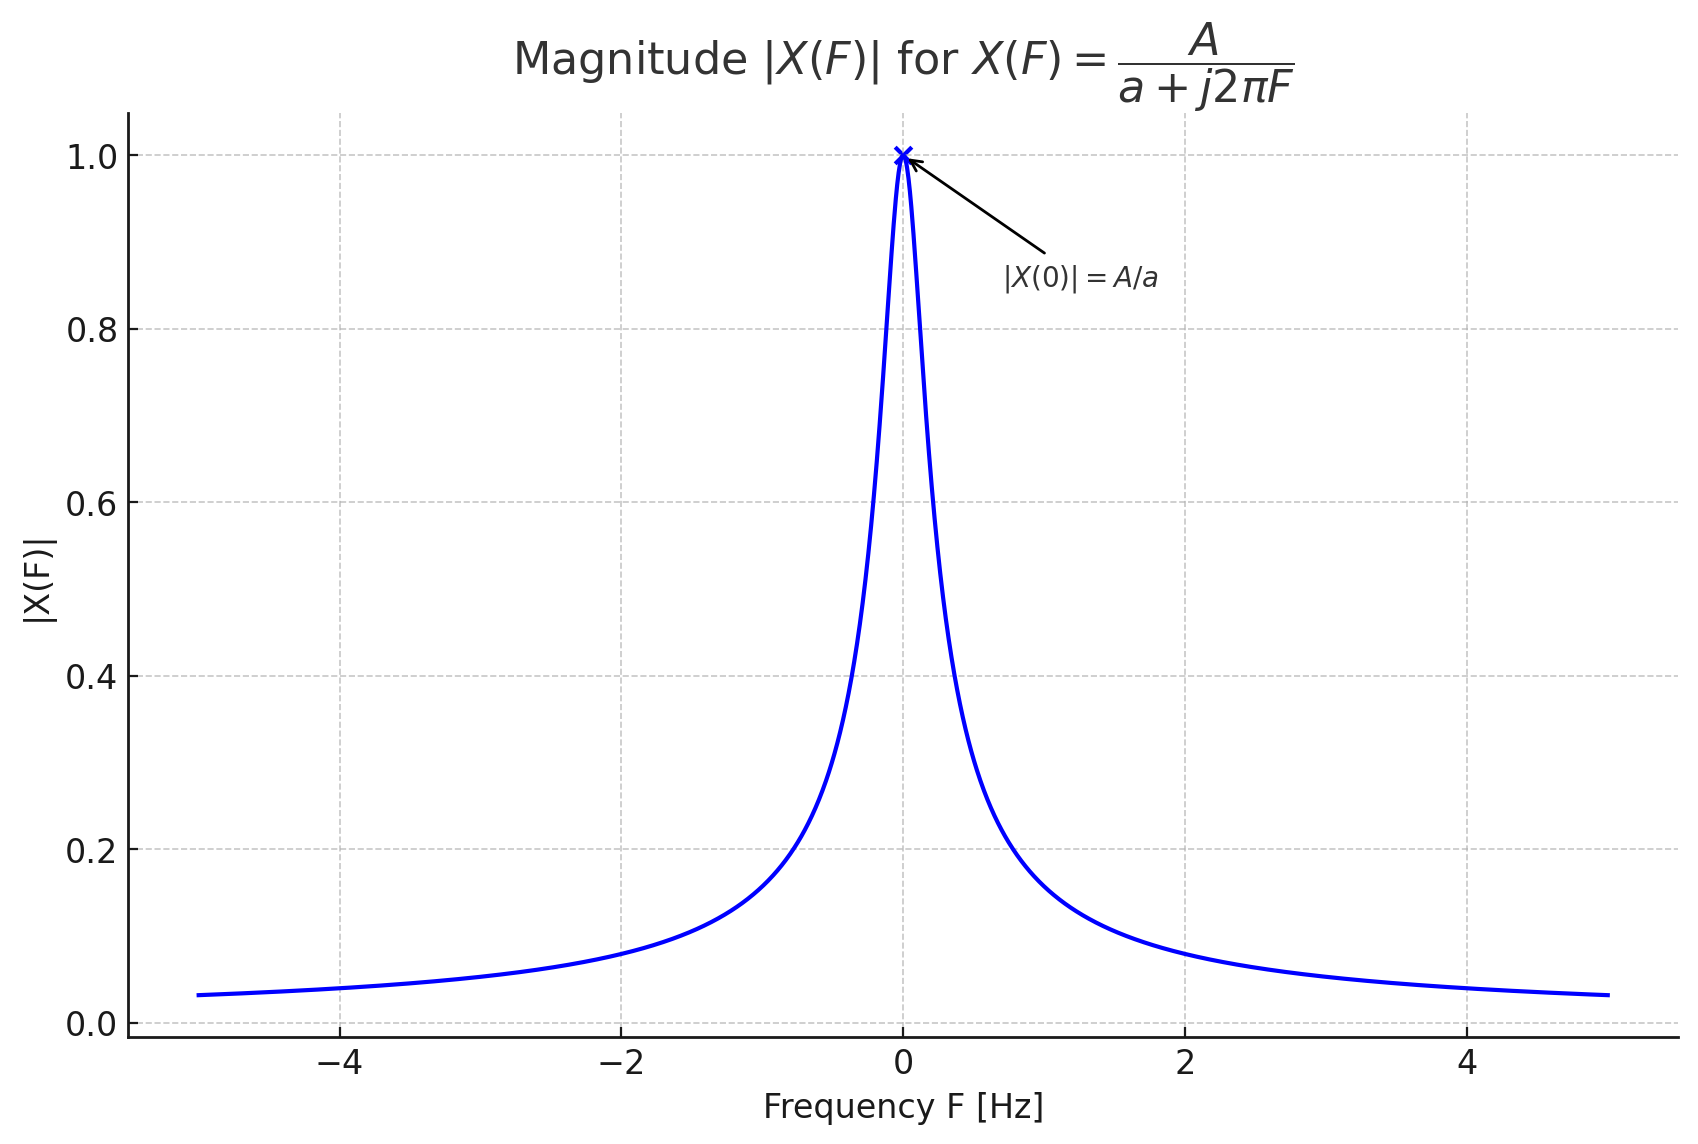
\includegraphics[width=0.6\textwidth]{Auxiliar_3_2}
        \captionof{figure}{Esquema}
      \end{center}
    De lo anterior, se puede concluir que el sistema es inherentemente inestable, puesto que los polos de lazo cerrado poseen una región en el semiplano derecho donde se pueden mover. Además, dado que los polos de lazo cerrado tienden a los ceros del plano, siempre existirá un polo de lazo cerrado inestable.
    \item \textbf{$K_A<0$:} Para $K_A<0$, se tiene un LGR conocido. Este corresponde a dos polos y un cero, que geométricamente se interpreta como una circunferencia centrada en el origen, con un radio igual a la distancia entre el cero y el punto medio entre los polos (el cual coincide con el punto de arranque). De esta forma, el LGR se ve de la siguiente forma:
    \begin{center}
        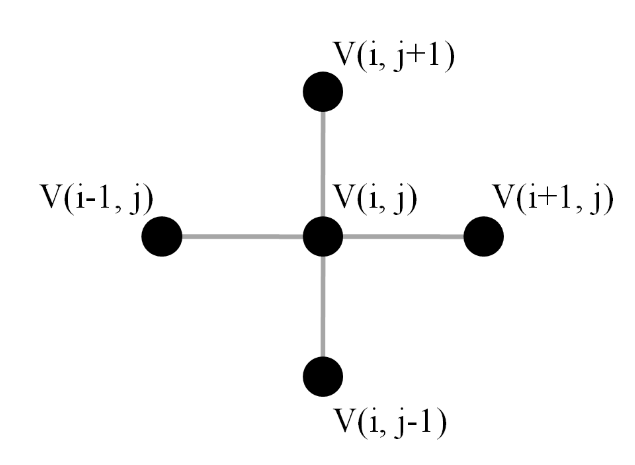
\includegraphics[width=0.6\textwidth]{Auxiliar_3_3}
        \captionof{figure}{Esquema }
    \end{center}
    A pesar de que existe LGR en el semiplano derecho, existe un valor de ganancia para el cual el sistema es estable. Esto es porque los polos de lazo cerrado pueden moverse por la circunferencia, por lo que eventualmente pueden estar en el semiplano izquierdo. Para encontrar este valor de ganancia, procedemos a plantear las condiciones de módulo y de ángulo:
    
    \begin{itemize}
        \item \textbf{Condición de ángulo:} Planteando la condición de ángulo:
        \begin{align}
            \sum \theta_i^p - \sum \theta_i^z &= 0^\circ \nonumber\\
            \theta_{-20K_T} + \theta_0 - \theta_{10K_T} &= 0^\circ \nonumber
        \end{align}
        Para encontrar la condición de inestabilidad, basta con entrar al punto del LGR donde la parte real es nula y solo se tiene una componente sobre el plano imaginario. De esta forma, los ángulos de las componentes están descritos por:
        \begin{align}
            \theta_{10K_T} &= 180^\circ - \arctan\left(\frac{h}{10K_T}\right) \nonumber\\
            \theta_{0} &= 90^\circ \nonumber\\
            \theta_{-20K_T} &= \arctan\left(\frac{h}{20K_T}\right) \nonumber
        \end{align}
        Reemplazando estos valores en la condición de ángulo se tendrá que:
        \begin{align}
            \arctan\left(\frac{h}{20K_T}\right) + 90^\circ - \left(180^\circ - \arctan\left(\frac{h}{10K_T}\right)\right) &= 0^\circ \nonumber\\
            \arctan\left(\frac{h}{20K_T}\right) + \arctan\left(\frac{h}{10K_T}\right) &= 90^\circ \nonumber
        \end{align}
    \end{itemize}
    Notar que la función $\arctan(x)$ tiende asíntoticamente a $90^{\circ}$ cuando $x\to \infty$. Bajo esta premisa, podemos afirmar que el argumento de la función trigonométrica debe tender hacie el infinito. Luego, si es que esta es una fracción, lo anterior significa que el denominador debe tender a 0. Es decir:
    \begin{equation}
        \lim_{x\to \infty}\arctan(x)=90^{\circ}\implies \frac{\frac{h}{20K_T}+\frac{h}{10K_T}}{1-\frac{h^2}{200K_T^2}} \to \infty \implies 1-\frac{h^2}{200K_T^2} \to 0 \nonumber
    \end{equation}
    Luego, como el denominador se debe anular, $1-\frac{h^2}{200K_T^2}=0$, por lo que $h=10\sqrt{2}K_T$. Con el valor de $h$, ya sabemos el punto en el eje imaginario donde el LGR cruza hacia el semiplano derecho. Finalmente, aplicamos la condición de módulo de manera geométrica.
    \item \textbf{Condición de módulo: } Aplicando la condición de módulo, debemos notar que la forma geométrica para calcularla nos da la ganancia total del sistema (es decir, la ganancia sistémica). Esto es muy importante a destacar, puesto que en nuestra planta teníamos un factor numérico que si debe ir incluido en la ganancia total del sistema. Si definimos $K_{sys}$ como la ganancia sistémica:
    \begin{align}
        G(s)H(s)&=\frac{K_A(s-10K_T)}{5s(s+20K_T)} \nonumber\\
        &=\frac{K_A}{5}\cdot\frac{(s-10K_T)}{s(s+20K_T)} \nonumber\\
        &=K_{sys}\cdot \frac{(s-10K_T)}{s(s+20K_T)} \nonumber
    \end{align}
    Aplicanod la condición de módulo:
    \begin{align}
        K_{sys}&=\frac{\Pi d_{i}^p}{\Pi d_{i}^z} \nonumber \\
        &=\frac{10\sqrt{2}K_T \cdot \sqrt{(20K_T)^2+200K_T^2}}{\sqrt{(10K_T)^2+200K_T^2}} \nonumber\\
        &=\frac{10\sqrt{2}K_T\cdot\sqrt{400K_T^2+200K_T^2}}{\sqrt{100K_T^2+200K_T^2}} \nonumber\\
        &=\frac{10\sqrt{2}K_T \cdot \sqrt{600K_T^2}}{\sqrt{300K_T^2}} \nonumber \\
        &=20K_T \nonumber
    \end{align}
    Finalmente, como $K_{sys}=20K_T$:
    \begin{align}
        K_{sys}&=20K_T \nonumber\\
        \frac{K_A}{5}&=20K_T \nonumber \\
        K_A&=20\cdot 5K_T \nonumber\\
        K_A&=100K_T \nonumber
    \end{align}
    Por lo tanto, la estabilidad se garantiza para $\abs{K_A}<100K_T$.
\end{enumerate}
\subsection*{Resolucion 1.3}
Suponga que el sistema de control experimenta una entrada del tipo $u(t)=400 + 60cos(\omega_0 t) + 2t$, con $\omega_0$ una frecuencia de resonancia constante ¿Cómo modificaría usted el controlador $K_A$ para alcanzar cero error a estado estacionario para dicha entrada?
En primera instancia, transformamos la entrada al dominio de laplace:
\begin{align}
    u(t)&=400+60 cos(\omega_0 t) + 2t \quad / \mathcal{L}(\cdot) \nonumber\\
    u(s)&=\frac{400}{s}+\frac{60}{s^2+\omega_0^2}+\frac{2}{s^2} \nonumber \\
    u(s)&=\frac{P(s)}{s^2(s^2+\omega_0^2)} \nonumber
\end{align}
Por el principio del modelo interno, para que un controlador pueda permitir alcanzar cero error en estado estacionario a una entrada $u(s)$, la función de transferencia del lazo directo debe tener el mismo denominador que $u(s)$. Por lo tanto, el controlador por lo menos debería tener en su denominador los términos $s^2(s^2+\omega_0^2)$. Sin embargo, debemos notar que esta condición se debe cumplir para la función de lazo abierto, y justamente la planta del sistema de control posee un integrador. De esta forma, par alcanzar c.e.e.e basta con agregar un denominador de la forma $s(s^2+\omega_0^2)$. Finalmente, el controlador debería tener la siguiente forma:
\begin{equation}
    G_c(s)=K_A\cdot\frac{\Pi (s+z_i)}{s(s^2+\omega_0^2)} \nonumber
\end{equation}
Notar que la función debe ser bipropia, por lo que el controlador debería tener ceros adicionales para cumplir este requerimiento. Para demostrar que efectivamente se cumple el c.e.e.e con este controlador, calculemos su error mediante el Teorema del Valor Final:
\begin{align}
    e&=\lim_{s\to 0 }\frac{sR(s)}{1+G(s)H(s)} \nonumber \\
    &= \lim_{s\to 0}\frac{s\frac{P(s)}{s^2(s^2+\omega_0^2)}}{1+K_A\cdot\frac{\Pi (s+z_i)}{s(s^2+\omega_0^2)} \cdot \frac{1}{s(s+K_T)}} \nonumber \\
    &=\lim_{s\to 0}\frac{\frac{P(s)}{s(s^2+\omega_0^2)}}{\frac{Q(s)}{s^2(s^2+\omega_0^2)}} \nonumber\\
    &=s\cdot \frac{P(s)}{Q(s)} \nonumber\\
    &=0 \nonumber
\end{align}
\end{solution}
    
    %%%%%%%%%%%%%%%%%%%%%%%%%%%
    %%%%%%%%%%%%%%%%%%%%%%%%%%%
    \question Considere la siguiente planta:
    \begin{align}
        G_{p}(s)= \frac{10}{(s^{2}+2s+3)}
    \end{align}
    \begin{enumerate}
        \item Diseñe un controlador proporcional (P) que le permita alcanzar una respuesta con un \textit{overshoot} o sobrepaso del 15\% y un tiempo de establecimiento al 2\% de 3.91 segundos.
        \item Diseñe un controlador proporcional integral (PI) que cumpla los mismos requerimientos solicitados en a).
        \item Calcule los errores en estado estacionario para los controladores anteriormente propuestos, ante una entrada escalón de magnitud $A$. Comente acerca de sus resultados.
    \end{enumerate}
    
    
%%%%%%%%%%%%%%%%%%%%%%%%%%%
\begin{solution}
\subsection*{Resolucion 2.1}
Diseñe un controlador proporcional (P) que le permita alcanzar una respuesta con un \textit{overshoot} o sobrepaso del 15\% y un tiempo de establecimiento al 2\% de 3.91 segundos.

A partir del enunciado podemos ver que se pueden obtener dos ecuaciones: una corresponde al sobrepaso y otra al tiempo de estabecimiento. De esta forma, podemos plantear el siguiente sistema de ecuaciones:
\begin{align}
    e^{-\frac{\xi \pi}{\sqrt{1-\xi^2}}}&=0,15 \label{eq_mov} \\
    t_s^{2\%}&=\frac{4}{\xi \omega_n} \label{eq_ts}
\end{align}
Manipulando la expresión (\ref{eq_mov}) podemos obtener lo siguiente:
\begin{align}
    e^{-\frac{\xi \pi}{\sqrt{1-\xi^2}}}&=0.15  \quad / ln(\cdot) \nonumber \\
    \frac{-\xi \pi}{\sqrt{1-\xi^2}}&=ln(0.15) \quad  / (\cdot)^2 \nonumber \\
    \frac{(-\xi \pi)}{1-\xi^2}&=ln^2(0.15) \nonumber\\
    (\xi \pi)^2&=(1-\xi^2)ln^2(0.15) \nonumber\\
    (\pi^2+ln^2(0.15))\xi^2-ln^2(0.15)&=0 \implies \boxed{\xi_{1,2}=\pm 0.5169} \nonumber
\end{align}
De los resultados obtenidos para el coeficiente amortiguamiento, elegimos el que es positivo puesto que es el que más tiene sentido en el problema. Así, reemplazando $\xi=0.5169$ en (\ref{eq_ts}) se tiene que:
\begin{align}
    3.91 &=\frac{4}{\xi\omega_n} \nonumber \\
    \omega_n&=\frac{4}{3.91\cdot0.5169} \nonumber \\
    \omega_n&=1.979 [\frac{rad}{s}] \nonumber
\end{align}
De esta forma, el punto de diseño estará dado por:
\begin{align}
    s_{1,2}&=-\xi \omega_n \pm j\omega_n \sqrt{1-\xi^2} \nonumber\\
    &=-0.5169\cdot 1.979 \pm j1.979\sqrt{1-0.5169^2} \nonumber \\
    &=-1.0229 \pm j1.6941
\end{align}
Luego, dado que necesitamos sintonizar un controlador proporcional, basta con aplicar la condición de módulo para encontrar la ganancia $K$. En efecto:
\begin{align}
    K&=\abs{\frac{1}{G(s)H(s)}}_{s=s^*} \nonumber \\
    &=\abs{\frac{1}{\frac{10}{(s^2 + 2s +3)}}}_{s=-1.0229+j1.6941} \nonumber\\
    &=0.0873
\end{align}
Finalmente, el controlador proporcional que permite cumplir con los requerimientos de diseño está dado por $K=0.0873$
\subsection*{Resolucion 2.2}
Diseñe un controlador proporcional integral (PI) que cumpla los mismos requerimientos solicitados en a).
Considerando los requerimientos de la parte a), debemos diseñar un controlador proporcional integral. La mayoría de estos controladores son funciones de transferencia bipropias, las cuales constan de una ganancia $K$, un cero $a$ y un polo $b$. De esta forma, proponemos el siguiente controlador PI:
\begin{equation*}
    G_c(s)=K\frac{(s+a)}{(s+b)}
\end{equation*}
Ahora bien, como se vió en la P1, la mayoría de los controladores se sintonizan para tener cero error en estado estacionario a cierta entrada. En este caso, es conveniente situar el polo de tal forma que nos permita alcanzar c.e.e.e a entrada escalón (puesto que es un PI, el cual solo tiene un polo). De esta forma, por el principio del modelo interno, deducimos que el controlador debe tener un polo ubicado en $b=0$. Así, $G_c(s)=K\frac{s+a}{s}$.\\
Con lo anterior, la función de lazo abierto va a estar dada por:
\begin{align}
    G(s)H(s)&=K\frac{(s+a)}{s}\frac{10}{(s^2+2s+3)} \nonumber \\
    &=K\frac{10(s+a)}{s(s+1+j1.4142)(s+1-j1.4142)} \nonumber
\end{align}
Con la función de lazo abierto anteirormente obtenida, sabemos que tenemos polos complejos conjugados. Además, debemos determinar los valores de $K$ y de $a$ para poder sintonizar de manera correcta el controlador. De manera visual, el problema se ve de la siguiente forma:
\begin{center}
    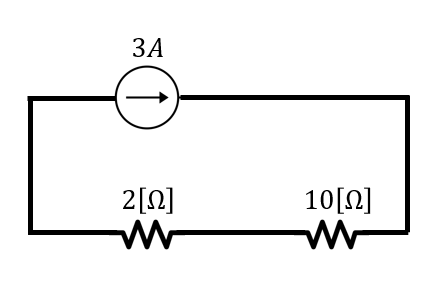
\includegraphics[width=0.5\textwidth]{Auxiliar_3_4}
    \captionof{figure}{Esquema}
  \end{center}
Notar que no sabemos realmente la posición del cero. Sin embargo, sin pérdida de generalidad, pueden asumir cualquier posición para este. Lo anterior es válido puesto que al desarrollar las ecuaciones podreán despejar dicho valor, y este será negativo o positivo dependiendo del sentido en el que se encuentre. \\
A partir de lo anterior, planteamos las condiciones de módulo y de ángulo:
\begin{enumerate}
    \item \textbf{Condición de ángulo: } la condición de ángulo para este LGR se ve de la siguiente forma:
    \begin{align}
        \sum \theta_i^p - \sum \theta_i^z&=180^{\circ} \nonumber \\
        \theta_0^p + \theta_1^p + \theta_2^p - \theta_a^z&=180^{\circ} \nonumber
    \end{align}
    Procedemos a calcular los ángulos correspondientes a los polos y ceros del sistema:
    \begin{align}
        \theta_1^p&=180^{\circ}-\arctan (\frac{1.6941-1.4142}{1-1.0229})=94.68^{\circ} \nonumber\\
        \theta_2^p&=180^{\circ}-\arctan (\frac{1.41421.6941}{1-1.0229})=90.42^{\circ} \nonumber\\
    \end{align}
    De esta forma, reemplazando estos ángulos en la condición anteriormente formulada llegamos al siquiente resultado:
    \begin{align}
        121.12^{\circ}+94.68^{\circ}+90.42^{\circ}-\theta_a^z&=180^{\circ} \nonumber \\
        \theta_a^z&=121.12^{\circ}+94.68^{\circ}+90.42^{\circ}-180^{\circ} \nonumber \\
        \theta_a^z&=126.22^{\circ} \nonumber
    \end{align}
    Por lo tanto, con este resultado, sabemos que el ángulo que describe $\theta_a^z$ debe ser mayor al ángulo descrito por el polo que se enceuntra en el origen. Luego, el cero debe ubicarse a la derecha del integrador y por ende en el semiplano derecho. De la misma forma, $\theta_a^z$ se puede expresar de la siguiente manera:
    \begin{align}
        \theta_a^z&=180^{\circ}-\arctan \Big(\frac{1.6941}{1.0229+a} \Big) \nonumber \\
        126.22^{\circ} &=180^{\circ}-\arctan \Big(\frac{1.6941}{1.0229+a} \Big) \nonumber \\
        arctan \Big(\frac{1.6941}{1.0229+a} \Big)&=180^{\circ}-126.22^{\circ} \quad /tan(\cdot)\nonumber\\
        \frac{1.6941}{1.0229+a}&=tan(53.78^{\circ}) \nonumber \\
        a&=\frac{1.6941}{tan(53.78^{\circ})}-1.0229 \nonumber \\
        a&=0.2179 \nonumber
    \end{align}
    Notar que $a$ tiene signo positivo, puesto que es la distancia que existe entre el origen y el cero. Sin embargo, el cero se encuentra ubicado en $a=0.2179$, por lo que al escribir la forma del controlador este debería ir como $s-a$, para lograr la ubicación deseada. De esta forma:
    \begin{align}
        G_c(s)&=K\cdot\frac{(s-0.2179)}{s} \nonumber
    \end{align}
    \item \textbf{Condición de módulo: }Por condición de módulo:
    \begin{align}
        K&=\abs{\frac{1}{\frac{10(s-0.2179)}{s(s^2+2s+3)}}}_{s=-1.0229+1.6941} \nonumber \\
        &=\abs{\frac{s(s^2+2s+3)}{10(s-0.2179)}}_{s=-1.0229+1.6941} \nonumber\\
        &=0.0822
    \end{align}
    Finalmente, el controlador queda como:
    \begin{equation}
        \boxed{G_s(s)=0.0822\cdot\frac{s-0.2179}{s}}
    \end{equation}
    Calcule los errores en estado estacionario para los controladores anteriormente propuestos, ante una entrada escalón de magnitud $A$. Comente acerca de sus resultados. 
Para calcular el error en estado estacionario de ambos controladores, basta con aplicar el Teorema del Final de Laplace. Este teorema se rige por la siguiente expresión:
\begin{equation}
    \lim_{t \to \infty}e(t)=\lim_{s \to 0}\frac{sR(s)}{1+G(s)H(s)} \label{TVF}
\end{equation}
donde $R(s)$ es el valor de la referencia. En este caso, la entrada es un escalón de magnitud $A$, por lo que $R(s)=\frac{A}{s}$.\\
Con lo anterior, procedemos a calcular el error para los controladores sintonizados en a) y en b):
\begin{enumerate}
    \item \textbf{Error del controlador P: }Evaluando el controlador proporcional en (\ref{TVF}) se tendrá que:
    \begin{align}
        e^{P}&=\lim_{s\to 0}\frac{s R(s)}{1+G(s)H(s)} \nonumber \\
        &=\lim_{s \to 0} \frac{s \cdot \frac{A}{s}}{1+0.0873\cdot \frac{10}{s^2+2s+3}} \nonumber \\
        &=\frac{3\cdot A}{0.0873\cdot 10} \nonumber \\
        &=0.775 A
    \end{align}
    Por lo tanto, el error en estado estacionario a una entrada escalón para el controlador proporcional es de un 77.5\%.
    \item \textbf{Error del controlador PI: }Evaluando el controlador proporcional integral en (\ref{TVF}) se tendrá que:
    \begin{align}
        e^{PI}&=\lim_{s\to 0}\frac{sR(s)}{1+ G(s)H(s)} \nonumber \\
        &=\lim_{s \to 0} \frac{s \cdot \frac{A}{s}}{1+10\cdot0.0822\frac{(s-0.2179)}{s(s^2+2s+3)}} \nonumber \\
        &=\lim_{s \to 0}\frac{A\cdot s \cdot (s^2+2s+3)}{s^3+2s^2+3s + 10\cdot0.0822(s-0.2179)} \nonumber \\
        &=0
    \end{align}
    Por lo tanto, el error en estado estacionario a entrada escalón para el controlador proporcional integral es 0. Como se podra anticipar, este resultado tiene sentido, puesto que el controlador incluye un integrador (se cumple el principio del modelo interno).
\end{enumerate}
\end{enumerate}
\end{solution}
%%%%%%%%%%%%%%%%%%%%%%%%%%%
\end{questions}
\newpage
%%%%%%%%%%%%%%%%%%%%%%%%%%%

\end{document}